\setlength\parindent{0pt}

\chapter{Methodology}

\section{Battery Performace Testing}
The battery consumption of an app depends a lot on the device, it’s make, operating system version, age, etc, especially for Android devices, of which there are thousands of different devices. In contrast, iOS runs only on iPhones, and thus there are very few different models. However, since we will be performing tests to determine usage patterns and battery demanding elements, we will not need the absolute battery consumption levels, and a general overview of the app’s battery consumption patterns will fulfil our requirements.\\

\textbf {Tests to Run:}
\begin{enumerate}
	\item Composing and sending emails (emails may contain attachments).
	\item Run Build Validation Test (BVT) for running basic app operations. (Build Verification test is a set of tests run on every new build to verify that build is testable before it is released to the test teams)
	\item Run detailed tests for problem areas discovered after running BVT tests 
\end{enumerate}
NOTE: These tests will be automated through scripts \\

Factors to be considered for Battery Performance Benchmarking:
\begin{itemize}
	\item Checking the battery status before the test begins.
	\item Enabling the location services for the application (if application requires).
	\item Starting the data sync of the application.
	\item Checking if the application is sending/receiving the data when in the background.
	\item Observing the battery consumption while performing the above supported features by the application.
\end{itemize}

To test battery performance, I will use a tool, Battery Historian, developed by Google. Battery Historian analyses a bugreport taken from an Android phone and shows detailed battery use statistics, including CPU and Kernel uptime, running process information, mobile network, WiFi, GPS, JobScheduler, SyncManager usage details, and usage statistics for each app (such as CPU and network usage information, wakelocks, services, etc) that was running in the duration for which the bugreport was taken.\cite{batteryhistorian} \\

For automation purposes, I will also develop a script which reports battery usage patterns, as Battery Historian has to be run manual. The tool will read the batterystats file and generate a HTML report showing wakelocks, wakeup alarms, jobs and syncs. I will also develop a script to generate a report showing difference in battery usage patterns for two versions of the app.

\begin{figure}[!h]
 	\begin{center}
		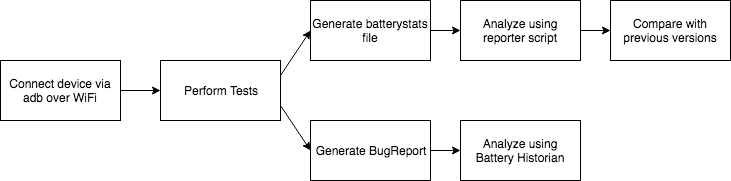
\includegraphics[scale=0.6]{Workflow}
		\caption{Workflow Diagram for Battery Performace Testing}
	\end{center}
\end{figure}

\section{Automated UI Testing}

To create a test case, first identify a use case that needs to be tested. Once we identify a use case, record the UI interactions required to complete the use case. Finally we write a test case to perform these interactions and verify if we have the desired result. The below example will illustrate this:\\

Suppose the use case is to compose and send an email with an attachment. The UI interactions to achieve this will be as follows:
\vspace{0.5cm}
\begin{figure}[!h]
 	\begin{center}
		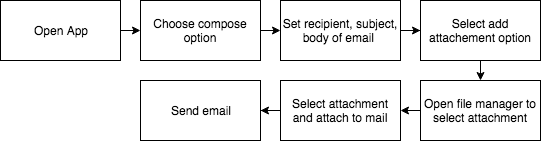
\includegraphics[scale=0.7]{uiflow}
		\caption{UI Interactions to compose and send a mail with attachment}
	\end{center}
\end{figure}

When writing the test case, we automated each and every one of the steps shown. We make use of UIAutomator library's python wrapper\cite{uiautomatordoc} to automate clicks, swipes and other UI interactions. The recipient is set to the same account that is sending the email, so that the received mail can be used to verify if the email was sent correctly. When the sent email is received, it is opened and checked for presence of attachment. The test can only pass on one condition: the email has the correct attachment. In any other case, like missing UI element, email not sent due to network error, wrong workflow logic, etc. will lead to failure.

\vspace{0.5cm}
\begin{figure}[!h]
 	\begin{center}
		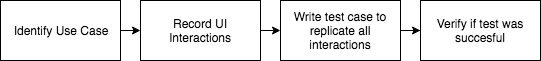
\includegraphics[scale=0.7]{Workflow2}
		\caption{Workflow Diagram for Automated UI Testing}
	\end{center}
\end{figure}